% Useful link: http://www.electronics-tutorials.ws/transistor/tran_1.html

\section{Modeling a BJT at DC}

\subsection{What \textit{is} a BJT?}

\subsubsection{The PN Junction}

There are two types of semiconductor: $p$ and $n$. $p$-type semiconductors have (positive) holes as their "free current carriers" whereas $n$-type semiconductors have (negative) electrons as their free current carriers.

A PN junction is formed when you place two pieces of $n$-type and $p$-type semiconductor together.

This PN junction is more classically known as a diode. Therefore the PN junction follows the diode equation.

\begin{equation}
\label{eqn-diode}
I_d = I_s \left(e^{(qV/kT)} - 1\right) \approx I_s \left(e^{(qV/kT)}\right)
\end{equation}

\subsubsection{The Bipolar Junction Transistor}

A BJT is formed of three sections of alternating semiconductor. NPN transistors are looked at in the course, for PNP transistors just reverse the polarity of the equations.

\begin{figure}[H]
\centering
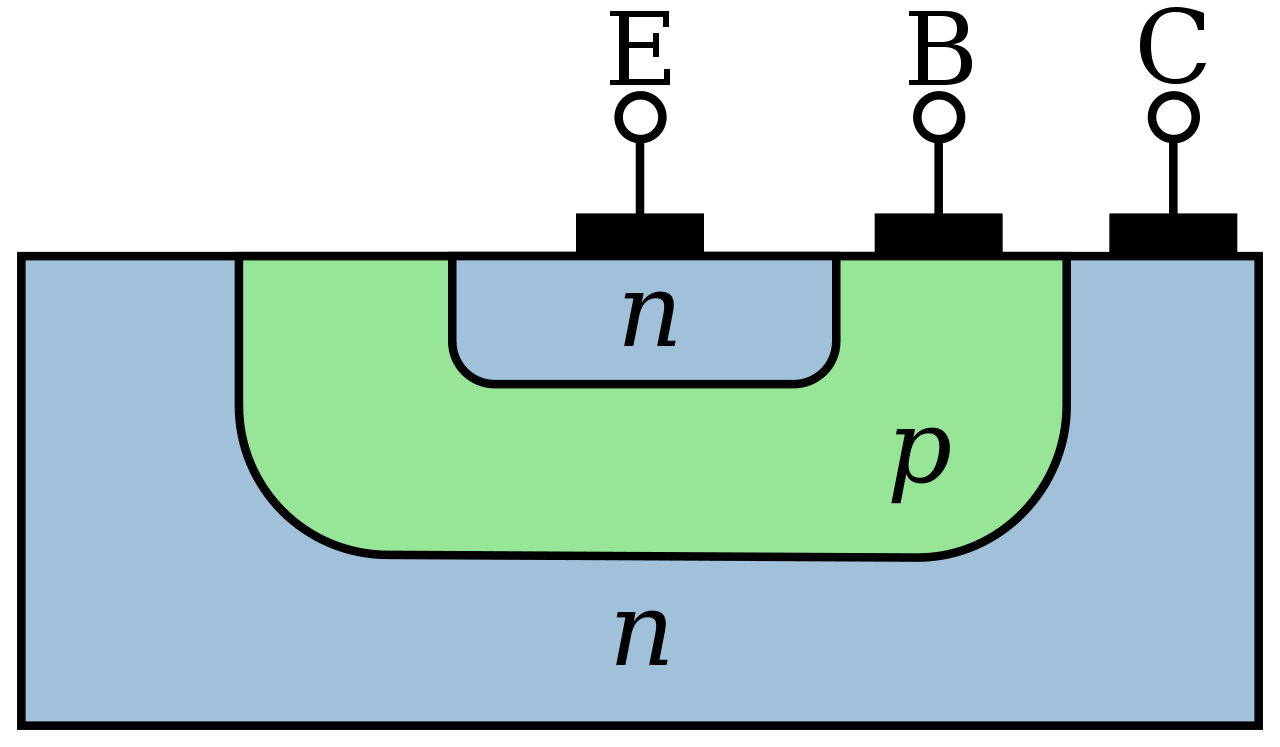
\includegraphics[width=0.25\textwidth]{images/npn-bjt-cross.png}
\caption{A realistic cross section of an NPN BJT.}
\end{figure}

BJT's have three connectors (emitter, base and collector) connected to each of the three sections of the transistor. In the connecting regions between each of the types of transistor there are depletion regions, like in the PN junction.

These depletion regions occur at the EBJ (\textbf{E}mmiter \textbf{B}ase \textbf{J}unction) and the CBJ (\textbf{C}ollector \textbf{B}ase \textbf{J}unction)

\subsection{Bias Conditions}

\begin{figure}[H]
\label{fig-active-bjt}
\centering
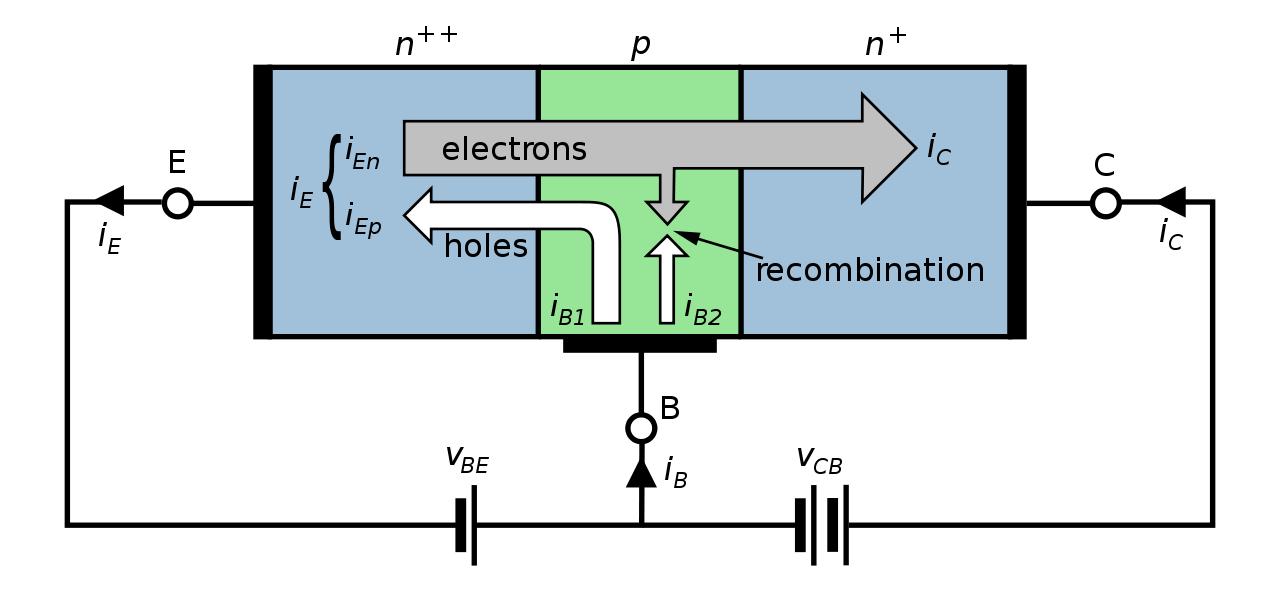
\includegraphics[width=0.5\textwidth]{images/npn-bias.png}
\caption{A biased BJT, annotated with arrows showing the direction of free current carriers in active mode.}
\end{figure}

When applying a voltage between the base and emitter ($V_be$) and the base and collector ($V_bc$) you get different characteristics.

\begin{table}[H]
	\centering
	\caption{Characteristics of a BJT based on bias conditions.}
    \begin{tabular}{lll}
     & EBJ Bias & CBJ Bias \\
    \hline
    Cut-off & Reverse & Reverse \\
    Active & Forward & Reverse \\
    Saturation & Forward & Forward
    \end{tabular}
\end{table}

\subsubsection{Current in a BJT for Active Mode}

As shown in figure~\ref{fig-active-bjt}, some recombination occurs at the base. This is a proportional current loss, therefore the current in the collector can be expressed as:

\begin{equation*}
I_C = \alpha I_E,\; \textrm{where } \alpha < 1
\end{equation*}

The term $\alpha$ is called the common-base current gain. When you connect a load across the collector and ground you get the following output voltage:

\begin{equation*}
v_o = RI_c = R\alpha I_E
\end{equation*}

Therefore, to get the largest output voltage we want to make alpha as close to 1 as possible. The amount of recombination is proportional to the number of holes (and therefore the doping level) in the base. As such, to get the maximum output voltage you must lightly dope the base.

\begin{table}[H]
	\centering
	\caption{Notation for doping levels in a semiconductor material, all levels are relative to the other semiconductors in the system.}
    \begin{tabular}{ll}
    $x^-$ & Lightly doped $x$-type semiconductor. \\
    $x^+$  & Heavily doped $x$-type semiconductor. \\
    $x^{++}$  & Very heavily doped $x$-type semiconductor.
    \end{tabular}
\end{table}

\subsection{Large Signal Equivalent}

For modeling a BJT at DC we use the "large signal equivalent" circuit.

\begin{figure}[H]
\centering
\href{https://en.wikipedia.org/wiki/Bipolar_junction_transistor#/media/File:Approximated_Ebers_Moll.svg}{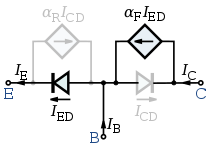
\includegraphics[width=0.3\textwidth]{images/large-signal.png}}
\caption{The large signal model of a BJT, with areas not included for active mode grayed out.}
\end{figure}

So from out large signal equivalent and what we already have determined about the current characteristics at bias we can form the following equations.

\begin{gather*}
I_E = I_s\left(e^{V_{BE}/v_T}\right) \\
I_C = \alpha I_E = \alpha I_s\left(e^{V_{BE}/v_T}\right) \\
I_B = I_E - I_C = (1-\alpha)I_s\left(e^{V_{BE}/v_T}\right)
\end{gather*}

From this we can see that for high values of $\alpha$ ($\alpha \approx 1$) we get a very small base current $I_B$, giving us a larger collector current $I_C$.

\subsection{The relationship between $\alpha$ and $\beta$}

The current gain, $\beta$ is the gain in current relating to the base and collector. It is normally on the order of 100.

\begin{gather*}
\textrm{Common-base Gain, }\alpha = \frac{I_C}{I_E} \\
\textrm{Current Gain, }\beta = \frac{I_C}{I_B} \\
\downarrow \\
\alpha = \frac{\beta}{\beta + 1},\; \beta = \frac{\alpha}{1 - \alpha}
\end{gather*}